%\documentclass[a4paper,10pt]{jarticle}
%\documentclass[]{jarticle}
\documentclass[10pt]{jarticle}

%\usepackage{graphicx}
\usepackage[dvipdfmx]{graphicx}
\usepackage{eclbkbox} %breakbox用
\usepackage{amsmath,amssymb}
\usepackage{verbatim}
\usepackage{moreverb}
\usepackage{ascmac,here,txfonts,txfonts}
\usepackage{listings,jlisting}
\usepackage{color}
\usepackage{fancybox}

%本文領域を広め(空白箇所マージン領域を小さめ)に設定
\lstset{
  breaklines = true,
  language=Python,
  basicstyle=\ttfamily\scriptsize,
  commentstyle={\itshape \color[cmyk]{1,0.4,1,0}},
  classoffset=1,
  keywordstyle={\bfseries \color[cmyk]{0,1,0,0}},
  stringstyle={\ttfamily \color[rgb]{0,0,1}},
  frame=tRBl,
  framesep=5pt,
  showstringspaces=false,
  numbers=left,
  stepnumber=1,
  numberstyle=\tiny,
  tabsize=2,
}

\setlength{\textwidth}{179mm}
\setlength{\textheight}{251mm}
\setlength{\topmargin}{-2cm}
\setlength{\oddsidemargin}{-1cm}
\setlength{\evensidemargin}{-1cm}

\begin{document}

\title{情報工学実験IIレポート(探索アルゴリズム1)}
\author{曜日&グループ番号: 月曜日&グループ0} %
\date{2014年12月14日}

\maketitle

\begin{abstract}
この骨組み(テンプレート)を利用する際には、
不要な箇所を削除した上で提出すること。
例えばこの要旨やコメント文の殆どは
「當間から学生へのコメント」であって、
「課題に対するレポート(報告書)」ではない。

このレポート(ファイル)は、「情報工学実験II・探索アルゴリズムその
1\cite{info2-search1}」の実験レポートの骨組みを例示している。
あくまでも例示であって、全てをこの通りに従う必要はないが、
指示された項目を含めた上で、
報告書として他者が読みやすいレポートとなるよう考慮すること。
\end{abstract}

\section*{グループメンバ}
(補足:レベル毎に \underline{全員が協力して実施} した上で、レベル毎にレポートをまとめる担当者を決め、全体を一つのレポートとして整理すること。分担方法も自由である。)
\begin{itemize}
 \item 945734J 當間愛晃: 担当Level1.1, 1.2
 \item 945700 hoge: 担当Level2.1, 2,2
 \item 945700 hoge: 担当Level2.3, 3.1
 \item 945700 hoge: 担当Level3.2
\end{itemize}

\section*{提出したレポート一式について}
レポート一式は
``\verb|shell:/net/home/teacher/tnal/2013-search1-mon/group0/|''
にアップロードした。
提出したファイルのディレクトリ構成は以下の通りである。

\vspace{+0.5cm}
(補足:必ず下記のように整理しろという指定ではない。
自分たちでやりやすいようにLevel毎に整理しても構わない)
\begin{breakbox}
\begin{verbatim}
./src/      # 作成したプログラム一式
./report/   # レポート関係ファイル.図ファイルを含む.
\end{verbatim}
\end{breakbox}

\newpage

\section{Leve l1: 探索とは}
\subsection{Level1.1: コンピュータと人間の違いを述べよ}
\subsubsection{課題説明}
コンピュータが人間より得意とするモノ、その反対に人間より不得手のモノ、両者について2つ以上の視点(立場や観点など)を示し、考察する。\\
\\
・コンピュータはパターン化されたものを決まった動作を繰り返す。\\
・コンピュータは大量の情報を取り扱いや特定のパターンに基づいてまとめたりする。\\
\\
・コンピュータの不得意なことは、感情移入判断することが出来ない、決まったことしか出来ない。\\
・コンピュータと違いは、パターン化されていないことも出来る
\subsubsection{考察}
\begin{itemize}
 \item 視点1: hoge\\
コンピュータならば**が可能であり云々\\
コンピュータは、パターン化されたことが得意\\
 \item 視点2: fuga\\
人間は**しなくてはならないため云々\\
人間は、パターン化されないことでも出来る
\end{itemize}


\subsection{Leve1.2: 評価方法(目的関数の設計指針や方法)について}
\subsubsection{課題説明}
Amazonにおける書籍検索時に「ファンタジー作品で泣ける作品」を探し出すため
のアイテム集合$x$と目的関数$f(x)$について検討した。

% アイテム集合x: 目的関数に入力されるxは何か?
% 目的関数f(x): 入力されたxをどのように評価したら良いか?
% (オプション) 上記で設計した目的関数の欠点があれば例示と共に解説せよ。

\subsubsection{アイテム集合$x$について}
%私達のグループはhogeをfugaすることについて検討を進めた。すなわち云々

我々のグループでは,ファンタジー作品のレビューに書いてあるワードをアイテム集合$x$とすることを考えた.
次のようなレビューを例にとると,レビューに書いてあるすべての単語がアイテム集合$x$になる.
\begin{quote}
いやぁ、おもしろい。
異世界ファンタジーと言うのは、最初の数ページでこれはちょっと、と思う場合と、そこ
で引き込まれてあっという間と言う場合の二種類がある気がするけど、本書はもちろん後
者の方。
ありえなぁいと叫ぶだけのような、そんな浅いファンタジーではなく、とてもとても重厚
な、しっかり細部も練り込まれた、実に味わい深い作品でした。
\end{quote}

\subsubsection{目的関数について}
目的関数$f(x)$はすべてのアイテム集合$x$(レビュー内容の単語)に対して
重み付けをし,それを足し合わせた合計を返す関数とする.
先ほどのレビューを例にとると,「おもしろい」や「重厚な」,「味わい深い」などの作品を高く評価する単語に対しては
他のワードより大きな値を付加する.
そして探索目的は値が最大になるような$f(x)$である(図\ref{fig:level1-2}参照).

% (補足:PDF図を挿入する例)

\begin{figure}[h]
	\begin{center}
		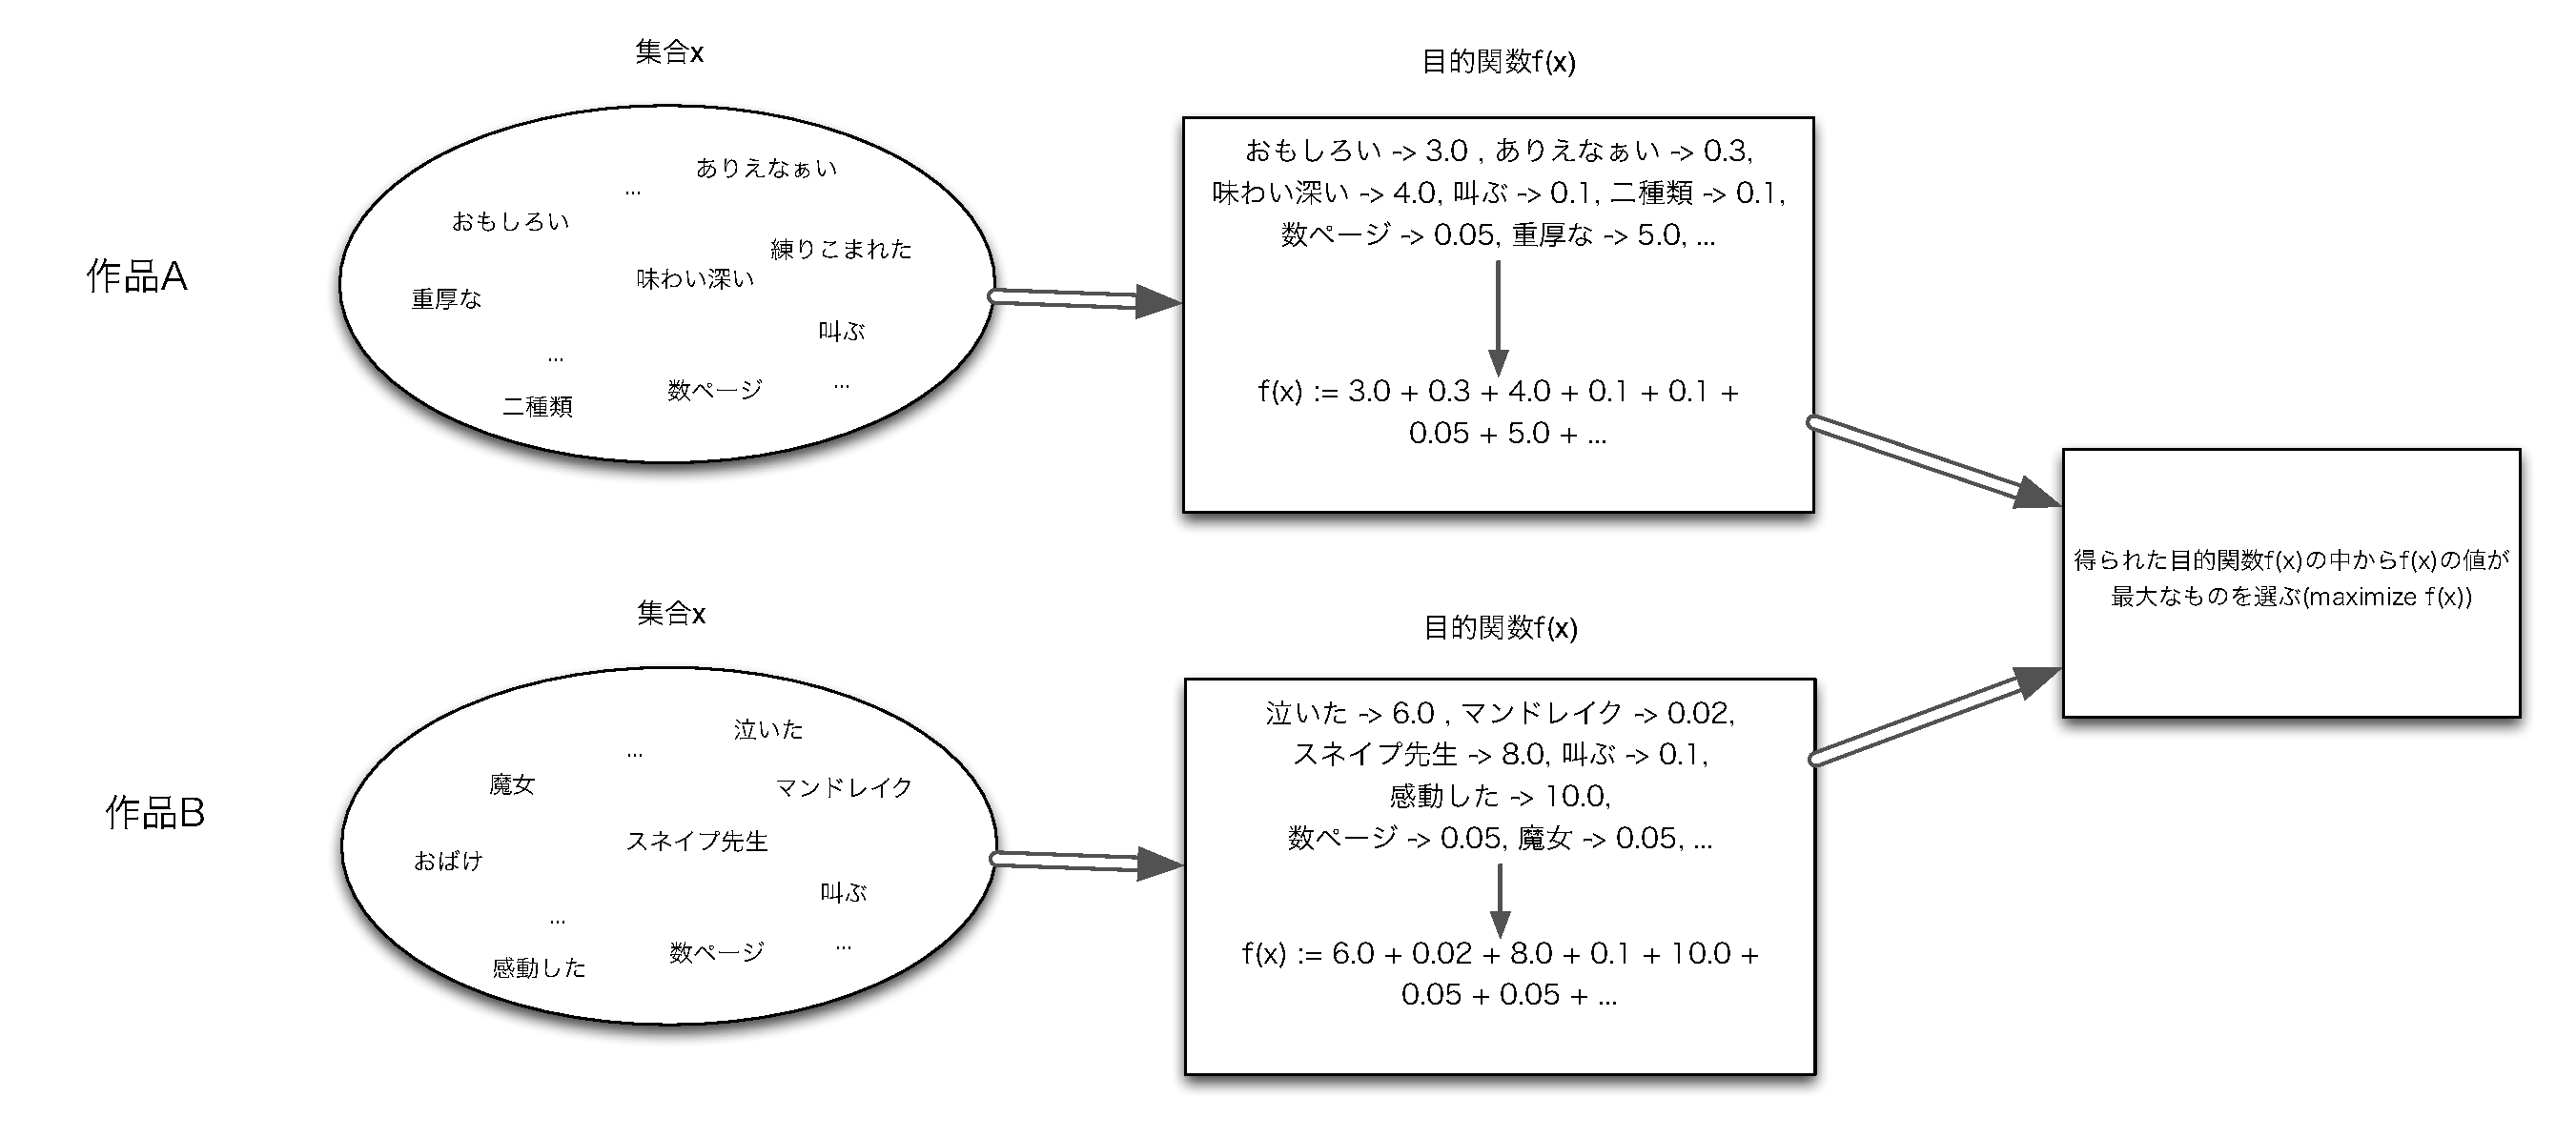
\includegraphics[scale=0.35]{./figs/level1-2.eps}
	\end{center}
	\caption{泣ける作品を探し出すまでの流れ}
	\label{fig:level1-2}
\end{figure}

\subsubsection{目的関数の欠点}
この目的関数の設計上の問題点は
あらかじめワードとワードに対応する重みの値を定義しておく必要があるということである.



\newpage

\section{Level 2: 最急降下法による最適化}
\subsection{課題説明}
3種類の連続関数$y=x^2$、$z=x^2+y^2$、$y=-x \times sin(x)$について、
最急降下法の適用を通して探索挙動を観察した。
以下ではまず共通部分である最急降下法の探索手続きについて、
フローチャートを用いて解説する。
その後、3種類の関数毎にプログラムの変更箇所、
観察意図観察方法、観察結果、考察について説明する。
\subsection{Level 2共通部分}

\subsubsection{探索の手続きとフローチャート(共通部分)}
\begin{figure}[htbp]
  \begin{center}
    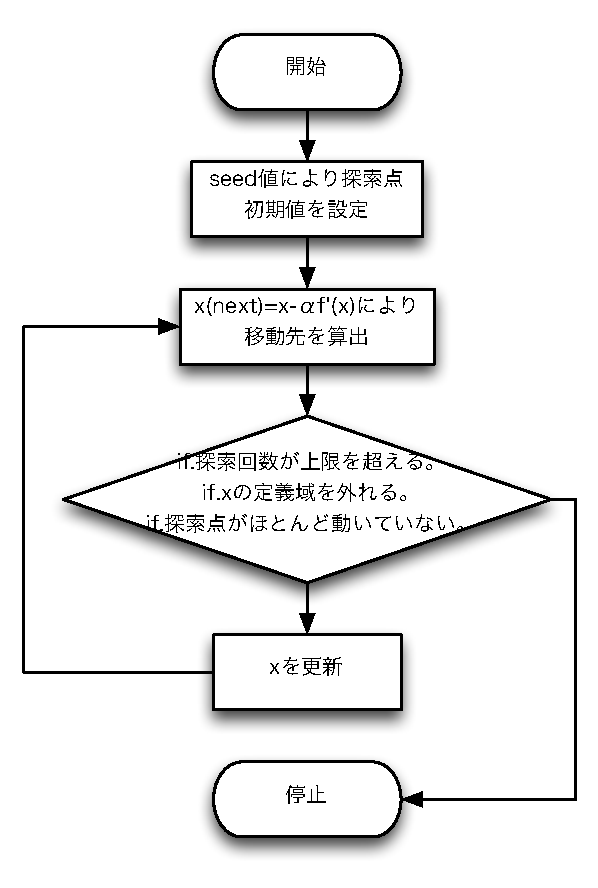
\includegraphics[clip,width=7.0cm]{./figs/tonal1.pdf}
    \caption{探索手続きのフローチャート}
 \end{center}
\end{figure}
 %共通部分の結果及び考察
\subsection{Level2.1: $y=x^2$ について}
\subsubsection{プログラムソース(変更部分)}
\subsubsection{観察意図と観察方法}
\subsubsection{実行結果}
\subsubsection{考察}


\subsection{Level2.2: $z=x^2 + y^2$ について}
\subsubsection{プログラムソース(変更部分)}
ソース変更:\\
/** 以下の式を編集して完成させよ(1) **/\\
 $ z = x*x + y*y$;\\
/** 以下の式を編集して完成させよ(2-1) **/\\
$z\_dx = 2*x$;\\
/** 以下の式を編集して完成させよ(2-2) **/\\
$z\_dy = 2*y$;\\
この三カ所である。\\
\subsubsection{観察意図と観察方法}
alphaの数字を変えてみて、どのようになるのかを確認して行く。\\
./trans\_xy\_vs\_func.sh''x**2+y**2''1を用いて、グラフの図を作成しどのようになっているのかを確信した。\\
\subsubsection{実行結果}
alpha = 0.1の時\\
/Users/e135711/実験2/steepestsearch ./trans\_xy\_vs\_func.sh''x**2+y**2'' 1\\
FINISH 3 step 75 x and y were not updated.\\
\\
alpha =1.0の時\\
/Users/e135711/実験2/steepestsearch ./trans\_xy\_vs\_func.sh ''x**2+y**2'' 1\\
FINISH 1 step 1000 this trial couldn't be search enough under the term\_cond=1000.\\
\\
\subsubsection{考察}
 x軸とy軸から見て“.data-1” using2:3:4を確認すると、alphaの数を変えてみた結果、数字を上げて行くと計算回数が少なくなり、数字を下げると計算回数が多くなった。\\

\subsection{Level2.3: $y=-x*sin(x)$ について}
\subsubsection{プログラムソース(変更部分)}
\subsubsection{観察意図と観察方法}
\subsubsection{実行結果}
\subsubsection{考察}



\newpage

\section{Level 3: 最急降下法が苦手とする状況}
\subsection{$B2]Bj@bL@(B}
$B:G5^9_2<K!$,6l<j$H$9$k>u67$K$D$$$F$=$NM}M3$r2r@b$7!"(B
$B8!F$$7$?2~A1J}K!$K$D$$$F2r@b$9$k!#(B

\subsubsection{$B860x(B}

\subsubsection{$B2~A1J}K!(B}

 %課題説明+提案解説
%\subsection{Level 3.1: $y = x^2 + (y^2)/10$ $B$K$D$$$F(B}
$B!V;3!JC+!W$N?t$O0l$D$K$b4X$o$i$:!"=PH/E@$N>l=j$K$h$C$F$O:GE,2r$K<}B+$9$k(B
$BC5:w2s?t$,BgI}$KA}$($F$7$^$&$3$H$,$"$kNc!#$=$NM}M3$H!"BP:v<jK!$K$D$$$F8!(B
$BF$$7$?!#(B

\subsubsection{$B860x(B}
\subsubsection{$B2~A1J}K!(B}


%\subsection{Level 3.2: $y = sqrt(abs(x))$ $B$K$D$$$F(B}
$BHyJ,2DG=$G$O$J$$2r(Bx$B$r4^$`Nc!#(B
$B$=$NM}M3$H!"BP:v<jK!$K$D$$$F8!F$$7$?!#(B

\subsubsection{$B860x(B}
\subsubsection{$B2~A1J}K!(B}


\newpage

\section{Level 4: モデル推定時における目的関数の設計}
Housing Data Set\cite{housingdata}を例に、
モデルの適切さを図るための目的関数に付いて設計した。

\subsection{目的関数について}
点と線の始端と終端の距離の和が小さければ小さいほど適切.
\subsection{設計理由について}
点と線の最短距離にしようと思いましたが.二点取った方がより正確になると思っ
たのでこちらにしました.

%\subsection{Level4.2: 嗜好モデルの構築方法}
\subsubsection{嗜好モデルの説明}
\subsubsection{上記モデルの利点および欠点}





\vspace{+1.0cm}
(補足:参考文献は thebibliography 環境を使って列挙し、
本文中で適切な箇所で引用するようにしましょう。
例えば下記文献は、アブストラクトやLevel 4で引用しています)
\begin{thebibliography}{99}
\bibitem{info2-search1}
情報工学実験2: 探索アルゴリズムその1(當間)\\
\verb|http://www.eva.ie.u-ryukyu.ac.jp/~tnal/2013/info2/search1/|
\bibitem{housingdata}
Housing Data Set\\
\verb|http://archive.ics.uci.edu/ml/datasets/Housing|
\end{thebibliography}

\end{document}
